\documentclass[10pt]{article}
\usepackage{tikz}
\usetikzlibrary{shapes.misc}
\usepackage[margin=0cm]{geometry}
\pagestyle{empty}
\tikzstyle{every node}=[cross out, draw, red]

\begin{document}

\vspace*{\fill}
\begin{center}
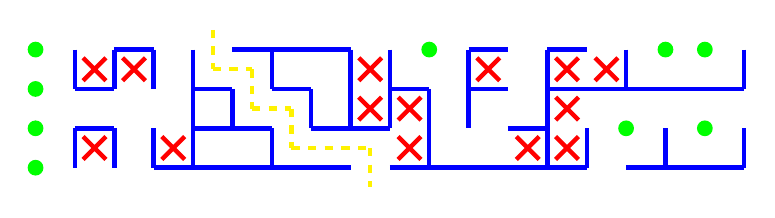
\begin{tikzpicture}[x=0.5cm, y=-0.5cm, ultra thick, blue]
% Walls
    \draw (2,0) -- (3,0);
    \draw (5,0) -- (8,0);
    \draw (11,0) -- (12,0);
    \draw (13,0) -- (14,0);
    \draw (1,1) -- (2,1);
    \draw (4,1) -- (5,1);
    \draw (6,1) -- (7,1);
    \draw (9,1) -- (10,1);
    \draw (11,1) -- (12,1);
    \draw (13,1) -- (18,1);
    \draw (1,2) -- (2,2);
    \draw (4,2) -- (6,2);
    \draw (7,2) -- (9,2);
    \draw (12,2) -- (13,2);
    \draw (3,3) -- (8,3);
    \draw (9,3) -- (14,3);
    \draw (15,3) -- (18,3);
    \draw (1,0) -- (1,1);
    \draw (1,2) -- (1,3);
    \draw (2,0) -- (2,1);
    \draw (2,2) -- (2,3);
    \draw (3,0) -- (3,1);
    \draw (3,2) -- (3,3);
    \draw (4,0) -- (4,3);
    \draw (5,1) -- (5,2);
    \draw (6,0) -- (6,1);
    \draw (6,2) -- (6,3);
    \draw (7,1) -- (7,2);
    \draw (8,0) -- (8,2);
    \draw (9,0) -- (9,2);
    \draw (10,1) -- (10,3);
    \draw (11,0) -- (11,2);
    \draw (13,0) -- (13,3);
    \draw (14,2) -- (14,3);
    \draw (15,0) -- (15,1);
    \draw (16,2) -- (16,3);
    \draw (18,0) -- (18,1);
    \draw (18,2) -- (18,3);
% Pillars
    \fill[green] (0,0) circle(0.2);
    \fill[green] (10,0) circle(0.2);
    \fill[green] (16,0) circle(0.2);
    \fill[green] (17,0) circle(0.2);
    \fill[green] (0,1) circle(0.2);
    \fill[green] (0,2) circle(0.2);
    \fill[green] (15,2) circle(0.2);
    \fill[green] (17,2) circle(0.2);
    \fill[green] (0,3) circle(0.2);
% Inner points in accessible cul-de-sacs
    \node at (1.5,0.5) {};
    \node at (2.5,0.5) {};
    \node at (8.5,0.5) {};
    \node at (11.5,0.5) {};
    \node at (13.5,0.5) {};
    \node at (14.5,0.5) {};
    \node at (8.5,1.5) {};
    \node at (9.5,1.5) {};
    \node at (13.5,1.5) {};
    \node at (1.5,2.5) {};
    \node at (3.5,2.5) {};
    \node at (9.5,2.5) {};
    \node at (12.5,2.5) {};
    \node at (13.5,2.5) {};
% Entry-exit paths without intersections
    \draw[dashed, yellow] (4.5,0.5) -- (5.5,0.5);
    \draw[dashed, yellow] (5.5,1.5) -- (6.5,1.5);
    \draw[dashed, yellow] (6.5,2.5) -- (8.5,2.5);
    \draw[dashed, yellow] (4.5,-0.5) -- (4.5,0.5);
    \draw[dashed, yellow] (5.5,0.5) -- (5.5,1.5);
    \draw[dashed, yellow] (6.5,1.5) -- (6.5,2.5);
    \draw[dashed, yellow] (8.5,2.5) -- (8.5,3.5);
\end{tikzpicture}
\end{center}
\vspace*{\fill}

\end{document}
